\section*{Variadische Funktionen mit Varargs}
	\begin{minipage}[t]{7.3cm}
		\begin{itemize}[noitemsep]
			\item Erlaubt beliebige Anzahl Parameter
			\item Nur am Schluss der Parameterliste erlaubt
			\item Compiler generiert ein Array
	\end{itemize}
	\lstinputlisting{code/varargs_call.java}
	\end{minipage}
	\hspace*{0.5cm}
	\begin{minipage}[t]{11cm}
		\vspace*{-0.2cm}
		\lstinputlisting{code/varargs_definition.java}
	\end{minipage}
\newpage
\section*{Spezielle Grundfunktionen}
Grundfunktionen sind Funktionen, welche in jedem \texttt{Object()} vorhanden sind und nach bedarf überschrieben werden können.
	\subsection*{Gleichheit}
		\texttt{equals()} ist standardmässig nur \textbf{Referenzvergleich}. Für einen inhaltlichen Vergleich muss \texttt{equals()} überschrieben werden. Bei der \texttt{String} Klasse ist es bereits implementiert, bei Arrays aber nicht!
	\lstinputlisting{code/equals.java}
	\subsection*{Hash-Code}
		\begin{itemize}[noitemsep]
			\item Sobald \texttt{equals()} überschrieben wird, muss auch \texttt{hashCode()} überschrieben werden.
			\item \texttt{hash-Code()} berechnet aus Objektinhalt den Hash-Code.
			\item Hashcodes müssen immer gleich sein, wenn Objekte equals sind.
			\item Umkehrung muss nicht umbedingt gelten!
			\item Mittels \textbf{Hashing} kann ein Element effizient gefunden werden.\vspace*{-0.15cm}
			\begin{itemize}[noitemsep]
				\item \textbf{Streuspeicher}: Elemente werden auf ein Array(Hash-Tabelle) verstreut, mit 'Hash-Code' als jeweiliger Index.
			\end{itemize}
		\end{itemize}
		\begin{minipage}[t]{8cm}
			\textbf{Eigene Hashfunktion:}
			\lstinputlisting{code/hashCode.java}
			Die Erstellung von \texttt{hashCode()} und \texttt{equals()} wird üblicherweise der IDE überlassen.
		\end{minipage}
		\hspace*{0.5cm}
		\begin{minipage}[t]{9.3cm}
			\textbf{Beispiel:}\\
			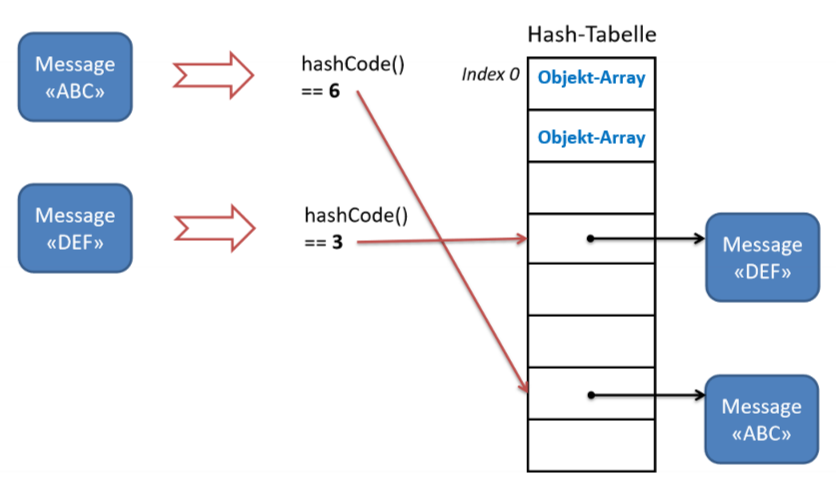
\includegraphics[height=6cm, align=t]{pics/hashing.PNG}
		\end{minipage}
		